\documentclass[margin = 10pt]{standalone}
\usepackage{tikz}
\usepackage{pgfplots} 
\pgfplotsset{compat = 1.18}

\begin{document}
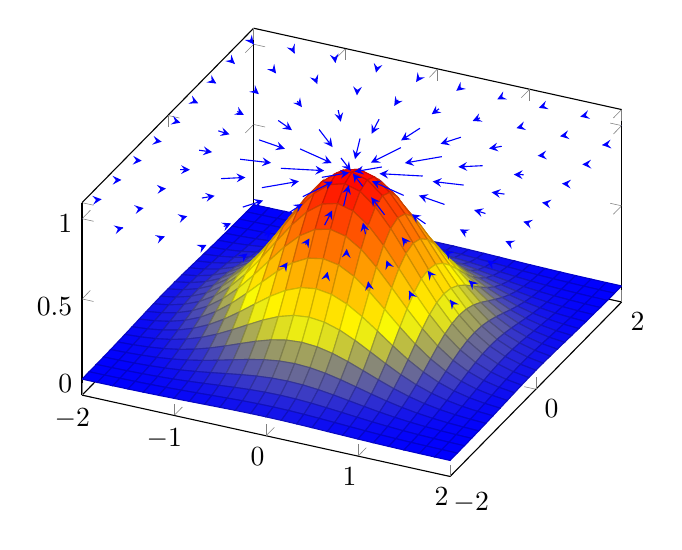
\begin{tikzpicture}
\begin{axis}[
    domain=-2:2,
    view={25}{45},
    ]
    \addplot3 [surf] {exp(0-x^2-y^2)} ;
    \addplot3 [
        blue,-stealth,samples=10,
        quiver={
            u={-2*x *exp(-x^2-y^2)}, %求x偏导
            v={-2*y *exp(-x^2-y^2)}, %求y偏导
            w={0},
            scale arrows=0.5
        }
    ] {1} ;
\end{axis}
\end{tikzpicture}
\end{document}
    